\begin{frame}{Bridge}
 \begin{center}
 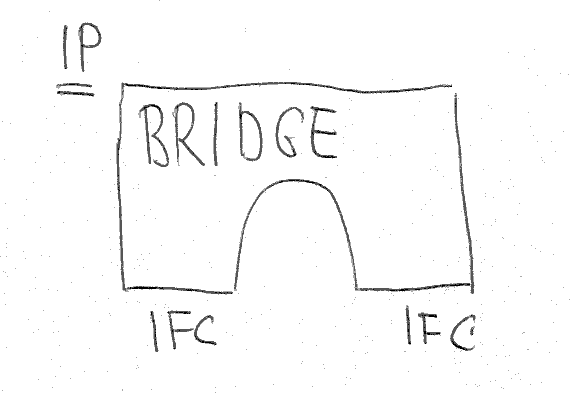
\includegraphics[width=0.5\textwidth]{bridge-picture.pdf}
 \end{center}
 \begin{itemize}
  \item {\em Bridge} wirkt wie ein {\em Interface} 
  \begin{itemize}
   \item hat eine IP-Adresse 
  \end{itemize}
  \item {\em Bridge} verbindet {\em Interface}'s {\bf IFC}
 \end{itemize}
\end{frame}

\begin{frame}{Bridge: \cod{brctl}}{Auf dem \host}
 \begin{itemize}
  \item Siehe \cod{tools/bridge.sh}
  \item Hole ip-addresse
  \item \cod{etc/resolv.conf}
 \end{itemize}
\end{frame}
